The aim of this section was not to prove that this vehicle was not a perpetual motion machine but to briefly explain its working principles. Literature detailing sufficient proofs have already been given by reliable sources for the scepticism about this concept to be considered unreasonable.

\begin{figure}[!htbp]
    \centering
    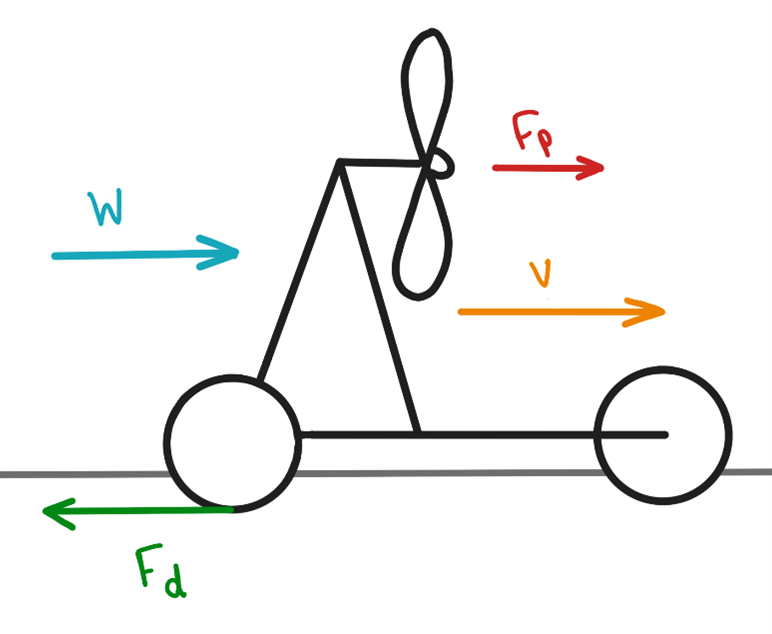
\includegraphics{images/part4/simplediag.png}
    \caption{Downwind Faster Than The Wind (DWFTTW) vehicle concept diagram}
    \label{fig:diagram}
\end{figure}

A Downwind Faster Than the Wind vehicle’s principle of operation is composed of four main events. First, the wind pushes the stationary vehicle. Second, the rotating wheels of the vehicle lead the chain connected to a propeller shaft. Third, the propeller spins and produces thrust. Approaching the wind speed, the propeller generates thrust even when the relative wind is zero, accelerating the vehicle until an equilibrium point between thrust and drag is reached. This point may be slower, equal to, or faster than the wind speed based on the efficiency of the vehicle components. It is important to emphasize that contrary to common belief, the rotor acts as a propeller producing thrust driven by the wheels, and is not a turbine extracting wind power to drive the wheels. This is the only difference between an upwind and a downwind vehicle as discussed earlier.

A set of equations were defined by Mark Drela in his “Dead Downwind faster than the wind analysis” \cite{drela20dead}. Where $F_p$ is the thrust provided by the propeller and $F_d$ is the force extracted from the ground as a result of the vehicle being pushed by the wind. The power outputted by the wheels and used by the propeller can be defined as follows. This introduces the overall propeller efficiency $\eta_p$.

\begin{equation}
P_{d}=F_{d} V
\label{eq:a}
\end{equation}

\begin{equation}
P_{p}=\frac{F_{p}(V-W)}{\eta_{p}}
\label{eq:b}
\end{equation}

Balancing both powers introduces a new efficiency coefficient $\eta_g$ which corresponds to the overall transmission efficiency between the wheels and the propeller.

\begin{equation}
    P_p = P_d \eta_g
    \label{eq:c}
\end{equation}

Substituting the forces defined in Equations \ref{eq:a} and \ref{eq:b} yields Equation \ref{eq:d} which is the simplified relationship between the propeller thrust and the wheel force:

\begin{equation}
F_{p}=F_{d} \frac{V}{V-W} \eta_{g} \eta_p
\label{eq:d}
\end{equation}

The net force on the vehicle is defined by Drela as the thrust generated by the propeller minus the force from the wheels. This leads to Equation \ref{eq:e} as follows:

\begin{equation}
    F_{net} = F_p - F_d
    \label{eq:fnet}
\end{equation}

\begin{equation}
F_{n e t}=F_{d}\left(\frac{V}{V-W} \eta_{g} \eta_{p}-1\right)
\label{eq:e}
\end{equation}

So long as the following coefficient is greater than one, the vehicle can be faster than the wind:

\begin{equation}
\frac{V}{V-W} \eta_{g} \eta_{p}>1
\label{eq:f}
\end{equation}

These equations highlight the importance of efficiency for the concept to achieve greater than wind speeds. One must note that Equations \ref{eq:d} and \ref{eq:e} are only defined for $V>W$. These equations use a simplified definition of the propeller efficiency $\eta_p$ which implies they are undefined for $W=V$. Workings to obtain the fully developed equation are available in \cite{drela20dead}.

